\documentclass[tikz,border=6pt]{standalone}
\usepackage[scaled]{helvet}
\renewcommand{\familydefault}{\sfdefault}
\usetikzlibrary{arrows.meta,positioning}

% ---------------- Colors ----------------
\definecolor{trainFill}{HTML}{E2EFDA}
\definecolor{trainDraw}{HTML}{92D050}
\definecolor{genFill}{HTML}{FFE5E5}
\definecolor{genDraw}{HTML}{FF0000}
\definecolor{discFill}{HTML}{DEEAF6}
\definecolor{discDraw}{HTML}{00B0F0}
\definecolor{backprop}{HTML}{ED7D31}
\definecolor{boxGray}{HTML}{7F7F7F}
\definecolor{subText}{HTML}{808080}

\begin{document}
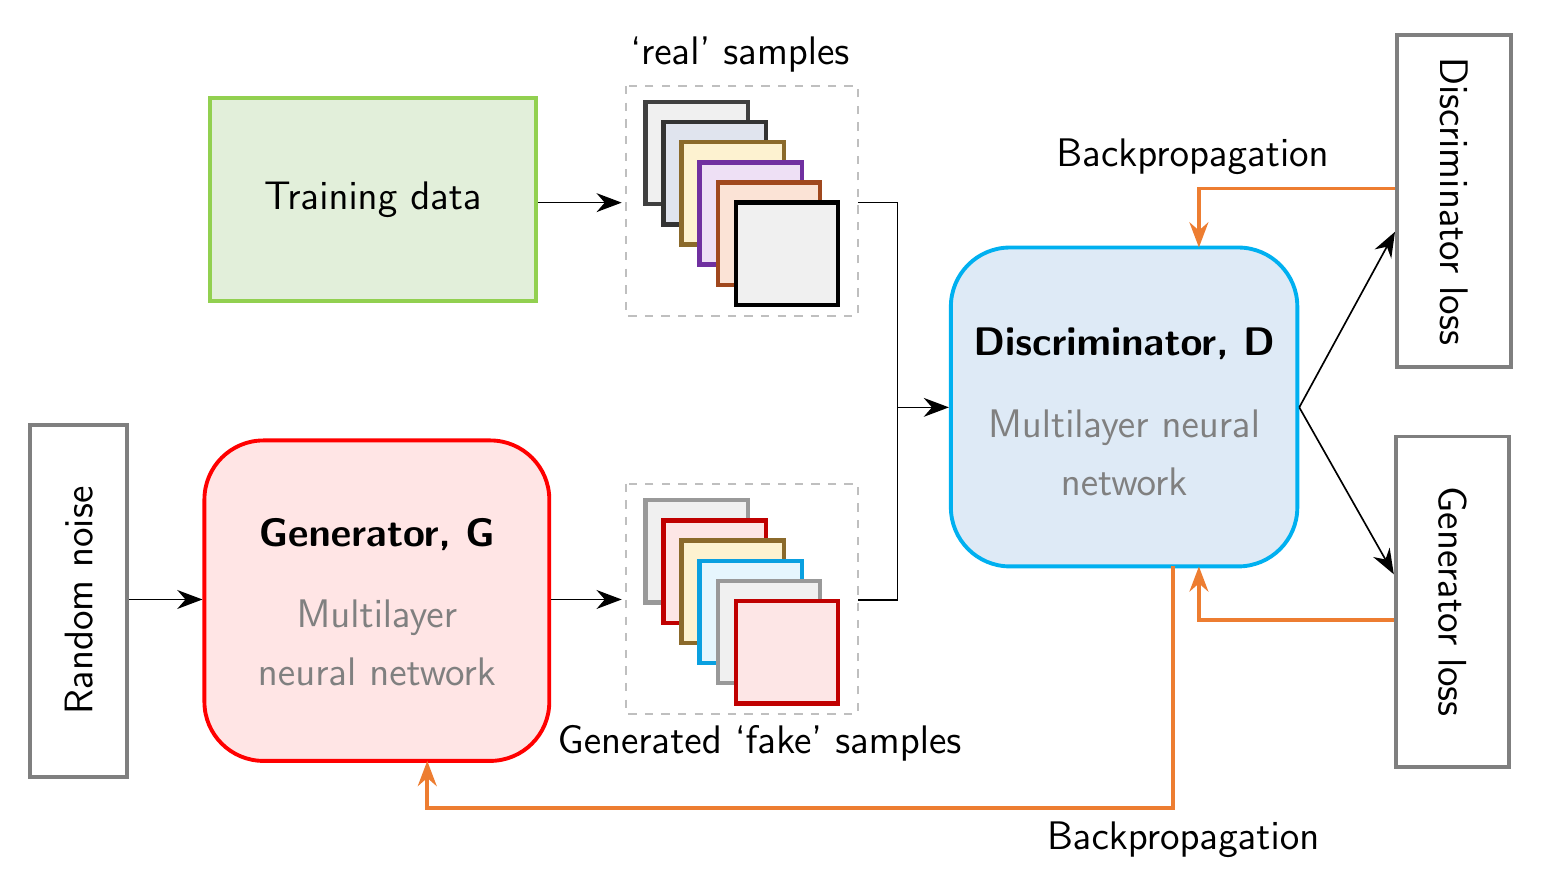
\begin{tikzpicture}[
    font=\Large,
    flow/.style={-{Stealth[length=3.2mm,width=2.4mm]}, line width=0.6pt},
    plain/.style={line width=0.6pt},
    bp/.style={-{Stealth[length=3.2mm,width=2.4mm]}, draw=backprop, line width=1.3pt},
    graybox/.style={draw=boxGray, line width=1.4pt, fill=white},
    samplebox/.style={draw=black!25, dashed, line width=0.8pt},
    sub/.style={text=subText, align=center, font=\Large}
]

% ---------------- Sample stack macro ----------------
% #1 = top-left x, #2 = top-left y, #3 = list of fill/draw pairs
\newcommand{\samplestack}[3]{%
    \foreach \f/\d [count=\k from 0] in {#3} {
        \pgfmathsetmacro{\sx}{#1 + 0.23*\k}
        \pgfmathsetmacro{\sy}{#2 - 0.256*\k}
        \filldraw[fill=\f, draw=\d, line width=1.6pt]
            (\sx,\sy) rectangle ++(1.3,-1.3);
    }%
}

% ---------------- Training data and real samples ----------------
\node[draw=trainDraw, fill=trainFill, line width=1.4pt,
      minimum width=4.14cm, minimum height=2.58cm] (train) at (4.69,8.76) {Training data};

\draw[samplebox] (7.9,10.2) rectangle (10.85,7.28);
\samplestack{8.15}{10.0}{
    black!6/black!75,
    {rgb,255:red,224;green,228;blue,238}/black!80,
    {rgb,255:red,253;green,242;blue,208}/{rgb,255:red,139;green,106;blue,43},
    {rgb,255:red,238;green,224;blue,245}/{rgb,255:red,112;green,48;blue,160},
    {rgb,255:red,251;green,227;blue,214}/{rgb,255:red,160;green,72;blue,30},
    black!6/black}
\node at (9.35,10.6) {`real' samples};
\draw[flow] (train.east |- 0,8.72) -- (7.85,8.72);

% ---------------- Random noise and generator ----------------
\node[graybox, minimum width=1.24cm, minimum height=4.47cm] (noise) at (0.95,3.665) {};
\node[rotate=90] at (noise.center) {Random noise};

\node[draw=genDraw, fill=genFill, line width=1.4pt, rounded corners=0.75cm,
      minimum width=4.38cm, minimum height=4.07cm] (gen) at (4.74,3.665) {};
\node[font=\Large\bfseries] at (4.74,4.5) {Generator, G};
\node[sub] at (4.74,3.13) {Multilayer\\[3pt]neural network};

\draw[flow] (noise.east |- 0,3.68) -- (gen.west |- 0,3.68);

% ---------------- Generated fake samples ----------------
\draw[samplebox] (7.9,5.15) rectangle (10.85,2.23);
\samplestack{8.15}{4.94}{
    black!6/black!40,
    {rgb,255:red,253;green,230;blue,230}/{rgb,255:red,192;green,0;blue,0},
    {rgb,255:red,253;green,242;blue,208}/{rgb,255:red,139;green,106;blue,43},
    {rgb,255:red,230;green,246;blue,253}/{rgb,255:red,10;green,160;blue,224},
    black!6/black!40,
    {rgb,255:red,253;green,230;blue,230}/{rgb,255:red,192;green,0;blue,0}}
\node at (9.6,1.85) {Generated `fake' samples};
\draw[flow] (gen.east |- 0,3.68) -- (7.85,3.68);

% ---------------- Discriminator ----------------
\node[draw=discDraw, fill=discFill, line width=1.4pt, rounded corners=0.75cm,
      minimum width=4.4cm, minimum height=4.05cm] (disc) at (14.23,6.125) {};
\node[font=\Large\bfseries] at (14.23,6.93) {Discriminator, D};
\node[sub] at (14.23,5.55) {Multilayer neural\\[3pt]network};

% merge of real and fake samples into D
\draw[plain] (10.85,8.72) -- (11.35,8.72) -- (11.35,3.67) -- (10.85,3.67);
\draw[flow] (11.35,6.12) -- (disc.west |- 0,6.12);

% ---------------- Loss boxes ----------------
\node[graybox, minimum width=1.45cm, minimum height=4.22cm] (dloss) at (18.42,8.74) {};
\node[rotate=-90] at (dloss.center) {Discriminator loss};

\node[graybox, minimum width=1.44cm, minimum height=4.2cm] (gloss) at (18.40,3.65) {};
\node[rotate=-90] at (gloss.center) {Generator loss};

\draw[flow] (disc.east |- 0,6.12) -- (dloss.west |- 0,8.35);
\draw[flow] (disc.east |- 0,6.12) -- (gloss.west |- 0,4.0);

% ---------------- Backpropagation paths ----------------
\draw[bp] (dloss.west |- 0,8.9) -| (15.18,8.15);
\node at (15.1,9.3) {Backpropagation};

\draw[bp] (gloss.west |- 0,3.42) -| (15.18,4.1);

\draw[bp] (14.85,4.1) |- (5.38,1.03) -- (5.38,1.63);
\node at (14.98,0.63) {Backpropagation};

\end{tikzpicture}
\end{document}
